\section{Tipi}

Rindkopa par to, kādi materiāli un ka ir mono un polikristāli un monokristāli labāki un kāpēc.

Darbā ir apskatīti divi Saules paneļu tipi. Ražotāju referenču lapās LG tiek prognozēta labāka atdeve saulainās dienās~\cite{LGtips}, bet JA labāka atdeve vājas gaismas intensitātes vidēs~\cite{JAtips}.

\begin{table}[h]
    \caption{JA un LG paneļu tipu salīdzinājums~\cite{JAtips}~\cite{LGtips}} % uzrakstīt kādu absolūto TSI izmērīja vai norādīt uz grafiku?
    \begin{center}
    \begin{tabular}{| r | c | c |}
    \hline
    Tips & JA & LG \\ \hline
    Modelis &  JAP60-275/4BB & LG365Q1C-A5\\ \hline
    % materiāls & silikons &   \\ \hline
	Kristāla veids & Polikristālisks & Monokristālisks \\ \hline
	% šūnas izmērs, mm  &156x156  & \\ \hline
	Šūnu skaits  &60  &60 \\ \hline
	Virsmas laukums, $m^2$ &1.64  &1.72 \\ \hline
	STC Pmax, $W$ 	&270 &365\\ \hline
	NOCT Pmax, $W$  &196 &275\\ \hline
	Efektivitāte, \% &16 & 20\\ \hline
    \end{tabular}
    \end{center}
    \label{tab:ja_lg_tipi}
\end{table}

Paneļu maksimālā jauda ($P_{max}$) tiek testēta pie:
\begin{itemize}
\item standarta testa nosacījumiem (\textit{Standart test condition} - STC):\\
Saules izstarojums 1000 W/m$^2$; apkārtējā temperatūra 25\textdegree C.
\item nominālās šūnas darba temperatūras (\textit{Nominal operating cell temperature} - NOCT):\\
Saules izstarojums 800 W/m$^2$; apkārtējā temperatūra 20 \textdegree C; vēja ātrums 1 m/s
\end{itemize}

% ielikt bildi ar to kas saules apstarojumā pazūd no imene

\section{Elektriskā shēma}

Šeit ir paskaidrots kas lācītim vēderā un kā tas strādā.
(buckle your seat-belts, cuz I'm gonna teach you something that I only learned two hours ago)

\begin{figure}[h]
    \centering
    \includegraphics[width=0.7\linewidth]{figures/misc/shema.pdf}
    \caption{Saules paneļu elektriskā shēma}
    \label{fig:paneli666}
\end{figure}

\section{Telpiskās orientācijas}

Kas kā kāpēc. \\

\begin{figure}[h]
    \centering
    \includegraphics[width=0.7\linewidth]{figures/misc/uzstadijumaShema.jpg}
    \caption{Saules paneļu telpisko orientāciju shēma}
    \label{fig:paneli}
\end{figure}

\begin{figure}[h]
    \centering
    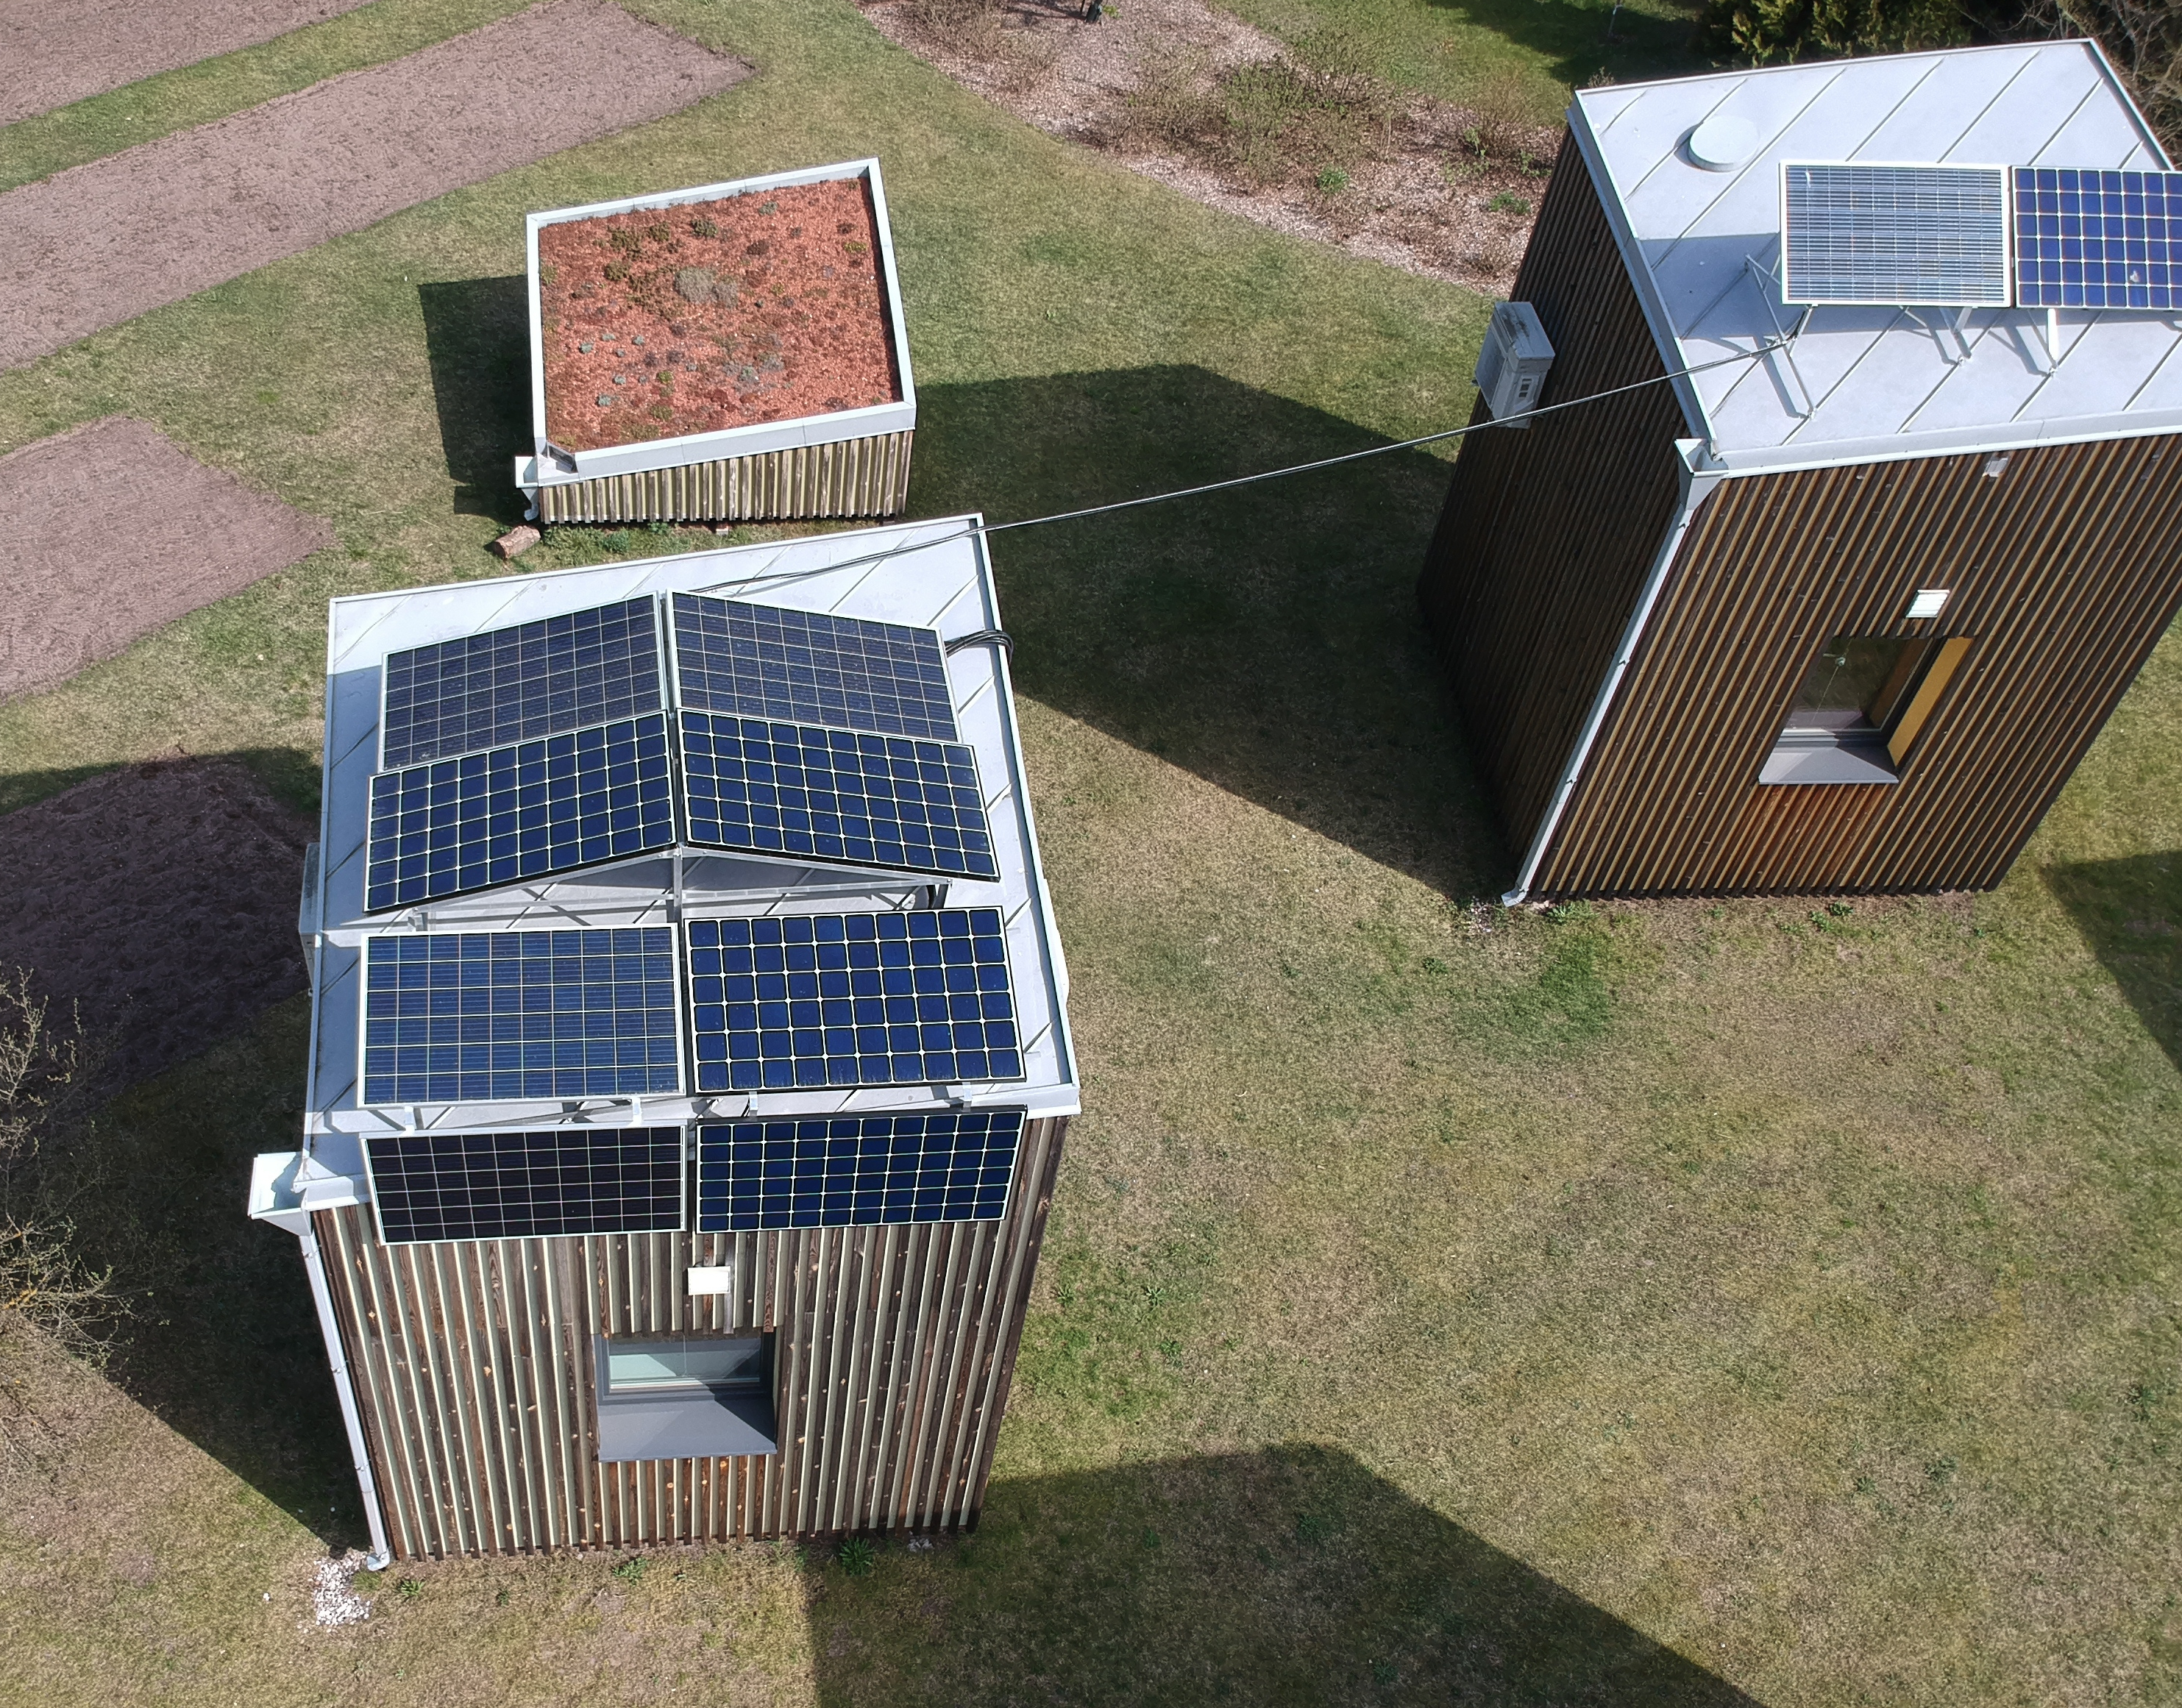
\includegraphics[width=0.7\linewidth]{figures/stenduBildes/overview2.JPG}
    \caption{Saules paneļu telpiskās orientācijas dabā (autors Māris Šinka)}
    \label{fig:paneli}
\end{figure}